% Select this file as the Overleaf main document to build the supplement.
\documentclass[10pt,twocolumn,letterpaper]{article}
\usepackage[review]{cvpr}
\newcommand{\mainref}[1]{\ref{main-#1}}
% Shared by main.tex and supplement.tex. Standard CVPR geometry is unchanged.
\usepackage[T1]{fontenc}
\usepackage{times}
\usepackage{amsmath,amssymb}
\usepackage{booktabs,multirow}
\usepackage{microtype}
\usepackage{algorithm}
\usepackage{algpseudocode}
\usepackage{xspace}
\usepackage{placeins}
\usepackage{needspace}
\newcommand{\ours}{\mbox{SE-JEPA}\xspace}
\newcommand{\base}{\theta_0}
\newcommand{\memory}{\mathcal{M}}
\newcommand{\replay}{\mathcal{R}}
\newcommand{\loss}{\mathcal{L}}
\newcommand{\R}{\mathbb{R}}
\DeclareMathOperator*{\argmin}{arg\,min}
\DeclareMathOperator*{\argmax}{arg\,max}
\newcommand{\missing}{\textemdash}
\newcommand{\best}[1]{\textbf{#1}}
\newcommand{\supref}[1]{Appendix~#1}
% References from the appendix to main-paper labels (supplement.tex redefines this for xr).
\providecommand{\mainref}[1]{\ref{#1}}
\hyphenation{AdaJEPA}
\setcounter{dbltopnumber}{2}
\graphicspath{{figures/}}
% Primitive input keeps LaTeX file hooks out of tabular alignment rows.
\makeatletter
\newcommand{\inputrows}[1]{\@@input #1 }
\makeatother

% Keep figure-only review pages aligned to the top.
\makeatletter
\setlength{\@fptop}{0pt}
\setlength{\@dblfptop}{0pt}
\makeatother

\usepackage{xr-hyper}
\definecolor{cvprblue}{rgb}{0.21,0.49,0.74}
\usepackage[pagebackref,breaklinks,colorlinks,allcolors=cvprblue]{hyperref}
\IfFileExists{main.aux}{%
  \externaldocument[main-]{main}%
}{%
  % Main-paper reference numbers for a fresh Overleaf import.
% Used only when main.aux is unavailable. Refresh after renumbering.
\newlabel{main-fig:condition_gains}{{4}{5}{}{figure.caption.5}{main.pdf}}
\newlabel{main-fig:deployment}{{7}{6}{}{figure.caption.8}{main.pdf}}
\newlabel{main-fig:efficiency_main}{{6}{6}{}{figure.caption.7}{main.pdf}}
\newlabel{main-fig:mixed14_learning}{{8}{7}{}{figure.caption.9}{main.pdf}}
\newlabel{main-fig:qualitative}{{3}{5}{}{figure.caption.4}{main.pdf}}
\newlabel{main-fig:teaser}{{1}{1}{}{figure.caption.1}{main.pdf}}
\newlabel{main-sec:mixed14}{{4.4}{7}{}{subsection.4.4}{main.pdf}}
\newlabel{main-tab:inheritance}{{3}{8}{}{table.caption.11}{main.pdf}}
\newlabel{main-tab:main}{{1}{5}{}{table.caption.3}{main.pdf}}
\newlabel{main-tab:mature_routing}{{5}{8}{}{table.caption.13}{main.pdf}}
%
}
\def\confName{CVPR}
\def\confYear{2027}
\title{SE-JEPA: Self-Evolving Latent World Models\\Supplementary Material}
\author{Anonymous CVPR submission}

% Link only the reference number, leaving the prefix and panels as text.
\DeclareRobustCommand{\paperxref}[3]{\mbox{#1~\ref{#2}#3}}
% Link only the letter in an appendix cross-reference.
\DeclareRobustCommand{\appendixref}[1]{\mbox{Appendix~\ref{#1}}}

\begin{document}
\maketitle
\appendix
\section{Implementation and Memory Management}
\label{app:implementation}

\paragraph{Compute environment.}
Model training and evaluation used a server with eight NVIDIA A100 GPUs.

\subsection{Fast and slow learning}
The label-free rigid-object configuration builds on the episodic adaptation loop of AdaJEPA~\maincite{wang2026adajepa}{35}. At every replan, recent observed transitions provide a self-supervised next-state prediction loss. One Adam step adapts the predictor's last block and the encoder's designated projection/head parameters in working copies, leaving the original pretrained weights fixed. The episode-local predictor and encoder changes are reset at the next episode. A retrieved slow predictor supplies the predictor initialization; it does not replace the frozen reference encoder.

Persistent replay is re-encoded by the reference encoder. Each slow learner is a full predictor copy, initialized from the pretrained predictor rather than from the final fast parameters of the episode that created the domain. For each slow optimization step, up to eight stored episodes are sampled with replacement; each contributes a random window of up to six latent frames. The prediction objective averages one-step observation-feature errors over the available history windows. Actions condition the prediction; the loss is computed only on observation features. Standard writes use 15 Adam steps. Founding a learner after $n$ stored episodes uses $15n$ steps to process the accumulated evidence. Merging likewise adds replay updates for absorbed experience.

\begin{table}[t]
  \centering
  \caption{Label-free configuration used for PushObj and PushT. The seven-round stream in \appendixref{app:additional} uses a slow learning rate of $2\times10^{-4}$ for all replay updates.}
  \label{tab:hyperparams}
  \small
  \begin{tabular}{lr}
    \toprule
    Setting & Value\\
    \midrule
    Fast predictor learning rate & $5\times10^{-4}$\\
    Fast encoder-head learning rate & $10^{-5}$\\
    Fast steps per replan & 1\\
    Recent adaptation buffer & 5 transitions\\
    Slow learning rate & $10^{-4}$\\
    Slow steps per standard write & 15\\
    Slow batch size (episodes) & 8\\
    Slow sampled window (frames) & up to 6\\
    Familiarity threshold $\tau_f$ & 0.0146\\
    Existing-domain cosine threshold & 0.10\\
    New-domain cosine threshold & 0.05\\
    Episodes to confirm a domain & 3\\
    Pending-pool capacity & 40\\
    Minimum episodes to train a learner & 3\\
    Retrieval window & first 3 replans\\
    Maturity history length $m$ & 3\\
    Maturity error-ratio threshold $\tau_m$ & 0.9\\
    Write rejection ratio & 1.2\\
    Merge evidence per direction & 2 episodes\\
    Merge relative tolerance & 0.5\\
    Fragment absorption interval & 25 episodes\\
    Absorption error-ratio threshold & 0.8\\
    Fragment-size limit & $<6$ episodes\\
    \bottomrule
  \end{tabular}
\end{table}

Replay stores compact latent trajectories rather than images. The pending pool is bounded, and merging and absorption remove redundant predictor copies as compatible domains are recognized.

\paragraph{Memory and computation.}
For $K$ domains, persistent model storage consists of $K$ slow predictor copies plus the frozen reference. Replay storage scales with the number of retained latent transitions, rather than the number of pixels in the original observations. Retrieval scores eligible predictors during the first three replans; slow optimization occurs after an accepted write, with 15 updates per standard write. Thus interaction efficiency and computation depend on different quantities: the former on replans until success, the latter on candidate count, retained experience, and replay updates. Domain merging shares both stored experience and a single surviving learner.

\subsection{Order of decisions}
Algorithm~\ref{alg:sejepa} summarizes a learning episode. Familiarity uses the geometric mean of newest-frame prediction errors on up to the first three observed transitions. The threshold is calibrated once on the shape backbone and transfers unchanged to the visual experiments.

\begin{algorithm}[t]
\caption{One deployment-learning episode of \ours}
\label{alg:sejepa}
\begin{algorithmic}[1]
  \Require Frozen $(E_0,P_0)$, memory $\memory$, initial observation $o$, goal $g$
  \State Reset fast parameters to $(E_0,P_0)$
  \State Initialize recent buffer $\mathcal{B}$ and episode trajectory $\tau$
  \While{budget remains and task is not complete}
    \State Optimize an action sequence with the current fast model
    \State Execute its first block; observe the next state
    \State Append real transitions to $\mathcal{B}$ and $\tau$
    \If{within the early retrieval window}
      \State Form candidates: $P_0$ and mature slow predictors
      \State Restrict to $P_0$ if the observed episode is familiar
      \State Select the smallest observed prediction error
      \State Load the selected predictor, retaining the fast offset
    \EndIf
    \State Adapt the fast model on recent real transitions
  \EndWhile
  \State Encode $\tau$ with frozen $E_0$
  \State Measure pre-update rollout errors of existing predictors
  \If{episode is unfamiliar}
    \State Propose a domain using retrieval or an update fingerprint
    \State Reject an incompatible write, or retain pending evidence
    \If{a domain is assigned or newly confirmed}
      \State Record validation before replay training when a learner exists
      \State Append latent experience; update its slow predictor
      \State Check bidirectional merges and periodic absorption
    \EndIf
  \EndIf
  \State Discard episode-local fast parameters
\end{algorithmic}
\end{algorithm}

The selected predictor's error is evaluated before it learns from the current episode, so maturity reflects transfer to data the predictor has not fitted. In read-only evaluation, the episode-end write, validation-history update, slow training, merging, and absorption steps are all disabled.

\subsection{Fingerprints and delayed domain founding}
A fingerprint concatenates the adapted predictor and encoder-head changes and is normalized to unit length. Domain prototypes accumulate normalized fingerprints from episodes planned from the reference; episodes starting from a slow predictor do not redefine that reference-based prototype. If an episode retrieved a slow predictor, its trajectory is first considered for that predictor's domain, subject to the error-ratio check before replay. Otherwise, it tries compatible domain directions in descending cosine order.

An unassigned episode enters a pending pool. It confirms a new domain when at least two pending fingerprints align with its own above the new-domain threshold. These members need not be pairwise aligned with one another; the incoming fingerprint is the common reference for this confirmation. The members and the new episode are transferred together to the new replay. No ground-truth shape or appearance category participates in this procedure.

\subsection{Merging and fragment absorption}
For a new unfamiliar episode, every existing trained learner is evaluated before training. The resulting ratios provide cross-domain evidence. Let $G_{A\to B}$ be the geometric mean error ratio of learner $B$ on recent episodes assigned to $A$, and $G_{A\to A}$ the corresponding ratio for learner $A$. Domains merge only if both directions satisfy
\begin{equation}
 G_{A\to B}\leq \min\{1,(1+\epsilon_m)G_{A\to A}\},
\end{equation}
with the symmetric condition for $B\to A$. Each direction requires two jointly evaluated episodes in the primary configuration. The larger domain retains its learner and incorporates the union of stored experience. Identifiers of merged domains remain retired for the rest of the stream.

Every 25 episodes, small immature domains can be absorbed into a mature predictor that explains their experience with an error ratio at most 0.8. The primary configuration limits absorption to fragments with fewer than six episodes and fewer than three maturity measurements. Pending-pool absorption and the additional absolute-error gate are disabled in the shape and visual experiments.

\subsection{Single-GPU deployment cost}
\label{app:deployment_cost}

To test deployment with a smaller compute and memory budget, we profiled Frozen, AdaJEPA, and \ours{} on a single consumer-grade NVIDIA RTX 4090. Each method and planner evaluated the same ten physical PushT tasks under seven visual conditions. We timed three repetitions per task--condition pair, yielding 1,260 measured episodes. All methods use the same implementation for each planner. In GD, CUDA graphs capture repeated optimization operations during warm-up to reduce kernel-launch overhead during planning.

\paragraph{Higher success with shorter episodes.}
Compared with AdaJEPA, \ours{} raises success by 34.3 percentage points under GD (32.86\% to 67.14\%) and 35.7 points under CEM (35.71\% to 71.43\%). Mean episode time falls by 26.7\% under GD (18.30 to 13.42 seconds) and 27.6\% under CEM (21.35 to 15.45 seconds). Peak allocated GPU memory increases by just 0.64\,GiB and 0.44\,GiB, respectively. \paperxref{Table}{tab:deployment_cost}{} reports all episodes and shows both allocated memory for live tensors and reserved memory, which includes the allocator cache.

\begin{table*}[t]
  \centering
  \caption{\textbf{Deployment cost on one RTX 4090 for matched PushT tasks.} Success (\%), mean replans, mean and P95 episode time (seconds), and maximum allocated/reserved GPU memory (GiB). Timing repetitions share the same tasks and learned memory.}
  \label{tab:deployment_cost}
  \small
  \begin{tabular}{@{}llrrrrrr@{}}
    \toprule
    Planner & Method & Success $\uparrow$ & Replans $\downarrow$ & Mean time $\downarrow$ & P95 time & Allocated & Reserved\\
    \midrule
    \inputrows{tables/deployment_cost.tex}
    \bottomrule
  \end{tabular}
\end{table*}

\paragraph{Timing protocol and runtime breakdown.}
The study evaluates reuse of memory learned after five rounds. Retrieval and fast adaptation remain active, with persistent memory fixed. We synchronize CUDA operations and exclude initialization and two warm-up episodes per run from timing. Episode time includes planning, adaptation, retrieval, simulator execution, and evaluation. We average repetitions within each task--condition pair before computing mean and 95th-percentile (P95) episode times. \paperxref{Table}{tab:deployment_phases}{} separates the major costs. Planning itself costs about 0.30 seconds per replan with GD and 0.44--0.45 seconds with CEM for all methods. The lower mean episode time comes from solving more goals with fewer replans. Compared with AdaJEPA, mean replans drop from 23.56 to 15.91 with GD and from 23.09 to 15.69 with CEM. Adaptation includes prediction diagnostics, and retrieval adds only 0.094 seconds per GD episode and 0.118 seconds per CEM episode on average. P95 episode time is higher for \ours: difficult episodes can still exhaust the budget while paying the additional adaptation and retrieval costs.

\begin{table*}[t]
  \centering
  \caption{\textbf{Mean episode time by component (seconds).} Adaptation includes diagnostics; simulator time includes evaluation. Minor reset and bookkeeping costs account for the remaining difference from \paperxref{Table}{tab:deployment_cost}{}.}
  \label{tab:deployment_phases}
  \small
  \begin{tabular}{@{}llrrrr@{}}
    \toprule
    Planner & Method & Planning & Adaptation & Retrieval & Simulator/evaluation\\
    \midrule
    \inputrows{tables/deployment_cost_phases.tex}
    \bottomrule
  \end{tabular}
\end{table*}

\paragraph{Learning and persistent storage.}
\paperxref{Table}{tab:deployment_memory}{} reports the preceding five-round learning stage, with 1,750 episodes per stream. Each final memory holds 733--766 trajectories in the profiled streams; their latent replay tensors occupy 21.5--22.9\,MiB. The full saved state also contains predictor and optimizer tensors, fingerprints, and pending experience. Across all six streams, consolidation uses 11,280--15,180 slow optimizer steps, including learner initialization, ordinary writes, merges, and absorption. These counts are reconstructed from the executed update rules and recorded events and reconciled with the saved replay states. The deployment timings above measure reuse of these learned memories; earlier consolidation is reported separately.

\begin{table*}[t]
  \centering
  \caption{\textbf{Memory after five learning rounds.} Active/mature predictor counts, retained trajectories, latent replay and full serialized state in MiB, and cumulative slow optimizer steps. Storage on disk is distinct from peak runtime GPU allocation.}
  \label{tab:deployment_memory}
  \small
  \begin{tabular}{@{}lrrrrrr@{}}
    \toprule
    Planner & Stream & Active/mature & Trajectories & Replay MiB & State MiB & Slow steps\\
    \midrule
    \inputrows{tables/deployment_memory.tex}
    \bottomrule
  \end{tabular}
\end{table*}

\section{Evaluation Protocols}
\label{app:protocols}

\subsection{Shape shifts}
The shape learning stream has five deployment rounds over seven shapes, with 50 episodes per shape in every round. The post-learning benchmark uses target seeds 2000, 2100, and 2200, each with 350 episodes. I, square, and small tee are unseen in pretraining; T, L, Z, and plus are seen.

For the paired planner comparison in \paperxref{Table}{tab:planners}{}, each planner has three learned memory states. Every state is evaluated on all three test seeds. For each seed we average over episodes and states, then compute the standard deviation across seed-level means. The single-seed PushObj baseline runs use test seed 2000.

\paperxref{Table}{main-tab:main}{} reports fifth-round online PushObj performance with adaptation and memory writing active: 844 successes out of 1,050 episodes (80.38\%) overall, and 329 out of 450 (73.11\%) on unseen shapes. \paperxref{Figure}{main-fig:teaser}{} reports the gains over AdaJEPA on held-out targets \mbox{after learning, for both GD and CEM}.

\subsection{Visual shifts}
The paired visual evaluation contains the original T condition, blur, salt-and-pepper noise, darkness, red agent, red object, and red goal. Three five-round learning chains resample targets every round, with 350 episodes per round. Held-out testing uses three target seeds and 50 episodes per condition. Direct checks of source-episode identifiers confirm that held-out sources never occur in the learning streams and that the three test seeds use disjoint sources.

The color-learning curve in \paperxref{Fig.}{main-fig:deployment}{} aggregates red-agent, red-object, and red-goal episodes. For each round and learning chain, it sums successes over the three conditions and divides by 150 episodes, and plots the mean of the three chain-level rates. The archived statistics include their sample standard deviation. The three conditions share the same 50 source targets within a chain and round.

For the VIS50 baseline comparison, we evaluate the same 50 initial/goal pairs under each of the six visual shifts, using planning seed 100.


\subsection{Success and interaction counts}
For the paired evaluations on PushObj and PushT, GD uses 100 optimization steps; CEM uses 10 iterations with 200 samples and 30 elites per iteration. On both datasets, success requires a joint Euclidean error below 20 simulator units across the pusher and object positions, and an object orientation error below $\pi/9$. Each executed model action contains five physical actions, and an episode has at most 30 MPC replans. For episode $i$ with success indicator $S_i$ and first successful replan $T_i$,
\begin{equation}
  \overline{T} = \frac{1}{N}\sum_{i=1}^{N}
  \big[\, S_i T_i + (1-S_i)\, T_{\max} \big], \qquad T_{\max}=30.
\end{equation}
Equivalently, $\overline{T} = T_{\max} - \sum_{t=1}^{T_{\max}-1} F(t)$, where $F(t)$ is the fraction of episodes solved by replan $t$; the cumulative curves in \paperxref{Fig.}{main-fig:efficiency_main}{} visualize $F$.

DINO-WM PushT CEM executes 25 actions per replan; \paperxref{Table}{main-tab:main}{} converts its mean to five-action units, $4.41\times25/5=22.05$, with failures assigned 30 units.

\subsection{Deformable manipulation}
\paperxref{Table}{tab:deform_hyperparams}{} summarizes the Rope and Granular learning and evaluation settings. In single-material consolidation, each pass revisits the same targets in the same order with the same planning seeds. The unseen-rope evaluation freezes the predictor saved after the first pass and tests it on 91 instances absent from the learning stream, against the frozen reference on the same instances. Mean CD falls from 0.664 with the reference to 0.349 with the one-pass predictor. Across the 91 matched instances, the predictor improves CD on 56. A paired percentile bootstrap over instances (20,000 resamples, seed 20261107) gives a 95\% interval of [0.162, 0.470] for the mean CD reduction. The observed mean reduction is 0.314.

\begin{table}[t]
\centering
\caption{\textbf{Rope and Granular hyperparameters.} Planning settings apply to both materials. Single-material consolidation uses a separate slow predictor for each material; mixed-material learning retains one memory across material switches.}
\label{tab:deform_hyperparams}
\footnotesize
\setlength{\tabcolsep}{3pt}
\begin{tabular}{@{}p{0.59\columnwidth}p{0.35\columnwidth}@{}}
\toprule
Setting & Value\\
\midrule
\multicolumn{2}{@{}l}{\textbf{Planning and evaluation}}\\
Backbone & DINO-WM\\
Planner & CEM\\
CEM samples / elites / iterations & 300 / 30 / 10\\
MPC replans / pushes per replan & 3 / 5\\
Maximum pushes per episode & 15\\
Evaluation metric & Final CD $\downarrow$\\
\midrule
\multicolumn{2}{@{}l}{\textbf{Single-material consolidation}}\\
Instances per material / passes & 50 / 4\\
Slow predictors per material & 1\\
Fast adaptation & Disabled\\
Slow learning rate & $10^{-4}$\\
Alternative slow learning rate & $2\times10^{-4}$\\
Unseen Rope instances & 91\\
Frozen predictor for unseen test & After pass 1\\
\midrule
\multicolumn{2}{@{}l}{\textbf{Mixed-material learning}}\\
Episodes per material / round & 50\\
Rounds / total episodes & 3 / 300\\
Consecutive episodes per material & 10\\
Optimizer & Adam\\
Fast steps per replan & 1\\
Fast predictor / encoder-head LR & $5\times10^{-4}$ / $10^{-5}$\\
Recent adaptation buffer & 5 transitions\\
Slow learning rate & $2\times10^{-4}$\\
Slow steps per standard write & 15\\
Slow batch size (episodes) & 8\\
Familiarity threshold & 0.117\\
Maturity history / error ratio & 3 / 0.9\\
Absolute write-error ratio limit & 20\\
\bottomrule
\end{tabular}
\end{table}

\begin{table*}[t]
 \centering
 \caption{Both planners on the paired post-learning evaluation sets. Shape All and Unseen use the separate PushObj test-seed streams. Visual All averages seven conditions and Shift six; visual Steps averages all seven conditions.}
 \label{tab:planners}
 \small
 \begin{tabular}{llcccccc}
 \toprule
 & & \multicolumn{3}{c}{PushObj} & \multicolumn{3}{c}{PushT}\\
 \cmidrule(lr){3-5}\cmidrule(lr){6-8}
 Planner & Method & All $\uparrow$ & Unseen $\uparrow$ & Steps $\downarrow$ & All $\uparrow$ & Shift $\uparrow$ & Steps $\downarrow$\\
 \midrule
 \inputrows{tables/paired_planners.tex}
 \bottomrule
 \end{tabular}
\end{table*}

\section{Baseline Implementations and Sources}
\label{app:baselines}

\paragraph{Model initialization.}
Frozen and AdaJEPA use the official task-specific checkpoints on PushObj and PushT. \ours uses task-trained ResNet world models; its PushObj backbone is trained for three epochs on 16,000 T, L, Z, and plus trajectories. The additional DINO-WM shape model uses the same trajectory count and epoch budget. Its updated PushT CEM checkpoint uses 16,000 newly generated random T-shape trajectories and epoch three. DreamerV3, IRIS, DINO CLS, and R3M use T-only checkpoints. DreamerV3 and IRIS are frozen offline world-model adapters for continuous-action CEM planning, without reward or policy learning. Configurations and source records are archived with the paper.

\paragraph{Evaluation groups.}
Frozen, AdaJEPA, and \ours use the paired held-out targets in \appendixref{app:protocols}. PushT Shift averages blur, noise, dark, red agent, red object, and red goal; Color averages the last three. The original condition enters the seven-condition curves. DreamerV3 and IRIS PushObj results use 50 targets per shape at seed 2000. The Unseen column consistently averages I, square, and small tee for all methods. Methods within each group share targets and the total action budget.

\paragraph{Published results and deformable references.}
The CDs for DreamerV3, IRIS, R3M, and DINO CLS are reported by Zhou et al.~\maincite{zhou2024dinowm}{42} on ten instances per task. Our DINO-WM and Frozen deformable rows share the same fixed reference on 50 instances. \appendixref{app:protocols} describes consolidation and the separate evaluation on unseen rope instances.

\section{Additional Results}
\label{app:additional}

\subsection{All object shapes}
\paperxref{Table}{tab:shape_domains}{} reports every held-out shape. \ours gives the largest gains on the unseen shapes: with GD, I rises from 44.7\% (AdaJEPA) to 77.6\% and square from 46.7\% to 61.1\%. It also leads on the seen shapes in aggregate.

\begin{table*}[t]
 \centering
 \caption{Held-out success (\%) per PushObj shape. I, square, and small tee are unseen in pretraining. All averages the seven shapes.}
 \label{tab:shape_domains}
 \small
 \begin{tabular}{llcccccccc}
 \toprule
 Planner & Method & I & L & Square & Z & Small tee & Plus & T & All\\
 \midrule
 \inputrows{tables/shape_domains.tex}
 \bottomrule
 \end{tabular}
\end{table*}

\subsection{All visual conditions}
\paperxref{Table}{tab:visual_domains}{} and \paperxref{Fig.}{main-fig:condition_gains}{} break the paired visual results down by condition. \ours improves on all seven conditions with both planners. The largest gains, more than 25 points, appear under red-object and red-goal recoloring, where episodic adaptation has to learn the same appearance correction again for each new target.

\begin{table*}[t]
 \centering
 \caption{Held-out visual success (\%) per condition on the paired targets. All averages seven conditions; Shift excludes Original.}
 \label{tab:visual_domains}
 \small
 \begin{tabular}{llccccccccc}
 \toprule
 Planner & Method & Original & Blur & Noise & Dark & Red agent & Red object & Red goal & All & Shift\\
 \midrule
 \inputrows{tables/visual_domains.tex}
 \bottomrule
 \end{tabular}
\end{table*}

\subsection{One memory across fourteen domains}
\label{app:mixed14}

This experiment places seven PushObj shapes and seven PushT visual conditions in one continual stream. The 14 domains form two recurring families, rather than all shape--appearance combinations. Each round presents all seven visual conditions followed by all seven shapes, with the shape order alternating between rounds. One memory state carries through every domain and round. Three chains per planner start with an empty memory and run for five rounds, with 50 episodes per domain per round. The same initial/goal pairs recur throughout; the changing seeds control run randomness. The curves measure continued learning on recurring goals; \mbox{\appendixref{app:protocols} evaluates held-out planning}.

\paragraph{Improvement across both families.}
Section~\mainref{sec:mixed14} and \paperxref{Figure}{main-fig:mixed14_learning}{} report five-round success averaged equally over GD and CEM. The figure's horizontal baselines average the archived evaluations, not additional five-round trajectories; shading is the sample SD of six planner-by-chain or planner-by-seed success rates. Each online round totals 4,200 episodes across both planners. The thumbnail strip shows the recorded initial observation of episode zero in each domain, from GD chain two in round five. Selection uses a fixed episode index independent of success; the native images retain the actual appearance corruptions. Both families improve from the first to fifth round: GD rises from 56.8\% to 69.1\% on visual conditions and from 74.4\% to 81.1\% on shapes; CEM rises from 57.6\% to 68.7\% and from 72.4\% to 82.9\%, respectively, with one memory retained throughout.

\paragraph{Final-round planning outcomes.}
\paperxref{Table}{tab:mixed14_summary}{} compares the fifth round of \ours with the archived Frozen and AdaJEPA baselines. \ours reaches 75.1\% (GD) and 75.8\% (CEM), with higher success in both families and fewer replans overall. Relative to AdaJEPA, the observed overall gaps are 10.0 and 10.4 percentage points, while all-episode replans decrease by 18.8\% and 17.6\%. These gains combine a higher fraction of solved goals with a lower interaction cost. \paperxref{Table}{tab:mixed14_domains}{} reports every domain: \ours exceeds AdaJEPA in 12 of 14 domains with GD, and in 13 with CEM, tying on noise.

Frozen retains the pretrained predictor, AdaJEPA adapts within each episode, and \ours retains predictive memory across the stream. The matched initial/goal pairs let us compare planning outcomes as \mbox{geometric and visual conditions recur}.

\begin{table*}[t]
 \centering
 \caption{\textbf{Mixed 14-domain online results.} Success (\%) and all-episode MPC replans, mean $\pm$ sample SD across three chains (\ours, round five) or three seeds (baselines). Each row has 2,100 episodes, split equally between the two families. Failures use the full budget.}
 \label{tab:mixed14_summary}
 \small
 \begin{tabular}{llcccc}
 \toprule
 Planner & Method & All success $\uparrow$ & Shape success $\uparrow$ & Visual success $\uparrow$ & Replans $\downarrow$\\
 \midrule
 \inputrows{tables/mixed14_summary.tex}
 \bottomrule
 \end{tabular}
\end{table*}

\begin{table*}[t]
 \centering
 \caption{\textbf{Mixed-stream success (\%) for every domain.} Each entry averages 150 episodes under the protocol of \paperxref{Table}{tab:mixed14_summary}{}. Original appearance and the T-shape block use different target sets and are retained as separate domains.}
 \label{tab:mixed14_domains}
 \small
 \begin{tabular}{llrrrrrr}
 \toprule
 & & \multicolumn{3}{c}{GD} & \multicolumn{3}{c}{CEM}\\
 \cmidrule(lr){3-5}\cmidrule(lr){6-8}
 Family & Domain & Frozen & AdaJEPA & \textbf{\ours} & Frozen & AdaJEPA & \textbf{\ours}\\
 \midrule
 \inputrows{tables/mixed14_domains.tex}
 \bottomrule
 \end{tabular}
\end{table*}

\subsection{Planning efficiency}
\paperxref{Figure}{main-fig:efficiency_main}{} plots cumulative held-out success against the number of MPC replans. \ours pulls ahead within the first four replans and keeps the lead for the rest of the budget, showing how the advantage develops before the full interaction budget of 30 MPC replans is exhausted.



\subsection{Deformable manipulation}


\paperxref{Figure}{main-fig:deployment}{} shows the four-pass learning curves in the main paper. \paperxref{Table}{tab:deform}{} adds standard errors to the deformable results of \paperxref{Table}{main-tab:main}{}. \paperxref{Table}{tab:deform_passes}{} follows consolidation pass by pass at two slow learning rates. With $10^{-4}$, CD decreases at every pass on both tasks. Rope improves faster in the early passes at $2\times10^{-4}$; the two learning rates yield similar final goal errors after four passes on both deformable tasks.

\begin{table}[t]
  \centering
  \caption{Deformable manipulation: mean CD $\pm$ standard error over 50 instances. \ours uses its slow predictor after four passes through the same 50 instances.}
  \label{tab:deform}
  \small
  \begin{tabular}{lcc}
    \toprule
    Method & Rope CD $\downarrow$ & Granular CD $\downarrow$\\
    \midrule
    \inputrows{tables/deform_rows.tex}
    \bottomrule
  \end{tabular}
\end{table}

\begin{table}[t]
  \centering
  \caption{CD of \textbf{\ours} after each consolidation pass at two slow learning rates (mean $\pm$ standard error, 50 instances).}
  \label{tab:deform_passes}
  \footnotesize
  \setlength{\tabcolsep}{2.5pt}
  \begin{tabular}{ccccc}
    \toprule
    & \multicolumn{2}{c}{lr $10^{-4}$} & \multicolumn{2}{c}{lr $2\times10^{-4}$}\\
    \cmidrule(lr){2-3}\cmidrule(lr){4-5}
    Pass & Rope & Granular & Rope & Granular\\
    \midrule
    \inputrows{tables/deform_passes.tex}
    \bottomrule
  \end{tabular}
\end{table}

\subsection{Mixed rope and granular learning}
\label{app:mixed_deformable}

We also test whether one persistent memory can separate and learn two deformable dynamics regimes in the simulated robot-arm environment. A single CEM chain alternates ten rope episodes with ten granular episodes, five times per round, for three rounds and 300 goals. Each round uses 50 goals per material, with no source trajectory shared across rounds. Both materials use the same rope-trained DINO-WM initialization, so granular is a new material for the pretrained predictor. Memory starts empty and persists across every material switch. Material labels are used only for analysis; the algorithm receives neither domain identities nor a prescribed number of domains.

This mixed-stream configuration retains fast adaptation and uses a slow learning rate of $2\times10^{-4}$. It also checks that an episode's prediction error is at most 20 times the candidate predictor's median error on its own stored trajectories before accepting a write. This absolute-error check supplements the relative validation test in \appendixref{app:implementation}. Each episode allows 15 pushes, and success requires final CD below 0.5 for rope or 0.2 for granular. These runs share one base and retain fast adaptation; the single-domain results use separate bases without fast adaptation.

\begin{table*}[t]
 \centering
 \caption{\textbf{Mixed deformable learning and domain separation.} One CEM chain, 50 new goal segments per material and round. Stored R/G counts are cumulative rope/granular members. Purity measures the fraction of stored members matching their domain's majority material. Correct retrievals count material-matched slow-predictor selections at MPC replans; selections of the frozen reference are excluded.}
 \label{tab:deform_mixed}
 \small
 \setlength{\tabcolsep}{5pt}
 \begin{tabular}{@{}crrrrrrr@{}}
 \toprule
 & \multicolumn{2}{c}{Rope} & \multicolumn{2}{c}{Granular} & \multicolumn{3}{c}{Memory and retrieval}\\
 \cmidrule(lr){2-3}\cmidrule(lr){4-5}\cmidrule(lr){6-8}
 Round & CD $\downarrow$ & Success (\%) $\uparrow$ & CD $\downarrow$ & Success (\%) $\uparrow$ & Stored R/G & Purity (\%) & Correct retrievals\\
 \midrule
 \inputrows{tables/deform_mixed.tex}
 \bottomrule
 \end{tabular}
\end{table*}

\paperxref{Table}{tab:deform_mixed}{} shows that the system discovers two mature memories and keeps them distinct: after three rounds, all 80 stored rope episodes and all 150 granular episodes belong to their respective material domains. The other 70 episodes are 69 familiar rope encounters and one rejected write. Stored-member purity is 100\% at every round endpoint. Of 660 slow-predictor selections, 653 (98.9\%) match the current material; all seven mismatches occur in the first round. All 457 slow-predictor selections in rounds two and three are material-matched, while the frozen reference remains available throughout deployment.

Mean final CD falls from 0.598 to 0.412 on rope and from 0.471 to 0.355 on granular across the three disjoint trajectory groups. Rope success rises from 60\% to 82\%; granular success is 2\%, 8\%, and 4\%. Together with material-correct retrieval, the decreasing goal distances show that one label-free memory can retain distinct dynamics and continue learning as materials alternate.

\subsection{Component protocols and learning rates}
\label{app:component_ablation}

\paperxref{Tables}{tab:gd_components_full}{} and \ref{tab:planner_components_full} use one five-round learning stream per task and planner. The final memory is tested with writes disabled on seeds 2000, 2100, and 2200, with 50 goals per domain and seed. Each cell summarizes 1,050 evaluations over seven domains. PushT includes the original appearance and six shifts. Replans average over all episodes, counting failures as 30; all ablations within a task \mbox{share the pretrained initialization}.

\paragraph{Memory design.}
The episodic-reset variant removes persistent memory. Direct inheritance carries fast weights to the next goal. The shared-replay variant trains one slow predictor on stored transitions; EMA instead averages fast parameters with mixing coefficient $\alpha=10^{-4}$. \paperxref{Table}{tab:gd_components_full}{} isolates these choices under GD. Replay exceeds EMA on both tasks, and domain-specific replay gives the highest success among these designs. Relative to direct inheritance, full \ours reduces mean replans from 16.12 to 11.37 on PushObj and from 22.33 to 12.93 on PushT.

\begin{table}[!ht]
 \centering
 \caption{\textbf{Memory-design ablations (GD).} Each entry reports success (\%) / all-episode MPC replans on 1,050 held-out goals. Variants share five learning rounds and paired test goals.}
 \label{tab:gd_components_full}
 \small
 \setlength{\tabcolsep}{3pt}
 \begin{tabular}{@{}lrr@{}}
 \toprule
 Variant & PushObj & PushT\\
 \midrule
 \inputrows{tables/gd_memory_design.tex}
 \bottomrule
 \end{tabular}
\end{table}

\paragraph{Planner consistency.}
\paperxref{Table}{tab:planner_components_full}{} evaluates the complete gate and learning-rate grid with both GD and CEM. Removing maturity screening changes which slow predictors can compete for retrieval, while preserving prediction-error selection. Removing familiarity protection allows familiar episodes to retrieve slow predictors and enter replay. The GD-only rows in \paperxref{Table}{tab:gd_components_full}{} also separate the read and write protections. The two mechanisms act at different stages: familiarity controls participation in memory, whereas maturity controls predictor readiness.

\begin{table*}[t]
 \centering
 \caption{\textbf{Gate and slow learning-rate ablations (GD and CEM).} Each entry is success (\%) / mean MPC replans over 1,050 held-out goals. The final state of one complete five-round learning stream is evaluated for each task and planner.}
 \label{tab:planner_components_full}
 \small
 \setlength{\tabcolsep}{5pt}
 \begin{tabular}{@{}lrrrr@{}}
 \toprule
 & \multicolumn{2}{c}{PushObj} & \multicolumn{2}{c}{PushT}\\
 \cmidrule(lr){2-3}\cmidrule(lr){4-5}
 Variant & GD & CEM & GD & CEM\\
 \midrule
 \inputrows{tables/planner_ablation_detailed.tex}
 \bottomrule
 \end{tabular}
\end{table*}

With either planner, removing familiarity protection improves PushObj but reduces PushT success. The maturity effect also depends on the planner: earlier retrieval benefits PushT GD, whereas screening benefits PushT CEM. A single fixed gate therefore offers a useful operating point across settings, with further gains possible through task-aware calibration that does not require domain labels. Across the learning-rate sweep, $5\times10^{-4}$ consistently performs worse than the default; the smaller rates preserve strong results with both optimizers.

\subsection{Transferring fast weights across goals}
We tested whether the parameter update from one episode helps on the next. Let $s_e$ be the offset from the pretrained weights at the start of episode $e$, and $\Delta_e$ the fast update in that episode. We set $s_{e+1}=s_e+w\Delta_e$, where $w=0$ resets to the pretrained model and $w=1$ retains the full update. Each variant sees the same 100 PushObj goals in five blocks of 20 (I, square, T, I, square). Keeping the full update loses more goals than it gains relative to reset (\paperxref{Table}{main-tab:inheritance}{}, two-sided exact McNemar $p=0.029$). Smaller weights give success rates closer to those of independent episodic reset.



\subsection{A seven-round shape stream}
A second PushObj stream runs seven rounds with a slow learning rate of $2\times10^{-4}$, one chain per planner. Each round has 50 episodes per shape, drawn without replacement and excluding the held-out sources, for 2{,}450 episodes per planner. Online success rises from 70.6\% in the first round to 78.6\% in the seventh with GD, and from 72.3\% to 78.3\% with the sampling-based CEM planner.

The episode logs record the fast-update fingerprint of every episode. \paperxref{Figure}{fig:directions}{} shows the cosine between consecutive fingerprints: the mean is 0.018 for both planners. Absolute cosine is below 0.1 for 96.3\% of GD pairs and 96.8\% of CEM pairs. These are descriptive statistics from one sequential stream per planner. These measurements support consolidating transition data rather than accumulating episode-specific parameter updates.

\begin{figure*}[t]
 \centering
 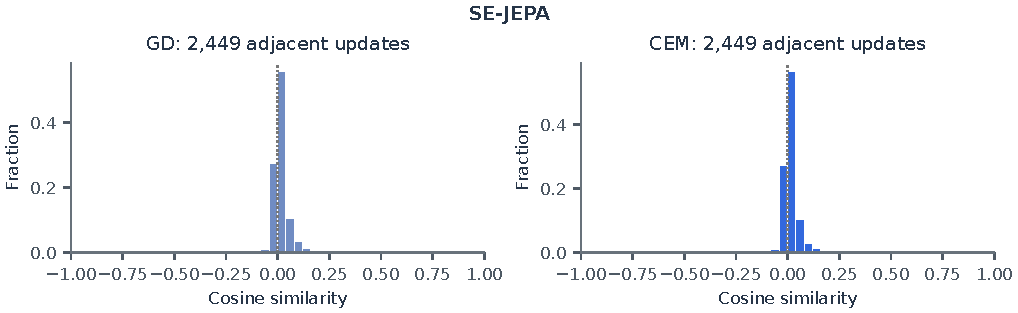
\includegraphics[width=\textwidth]{update_directions.pdf}
 \caption{Cosine similarity between consecutive fast-update fingerprints in the seven-round shape stream (2{,}449 pairs per planner).}
 \label{fig:directions}
\end{figure*}

\subsection{Memory use across episodes}
\label{sec:selectivity}

\ours learns selectively. In a seven-round PushObj stream of 2{,}450 episodes per planner, it writes only 25\% (GD) to 27\% (CEM) of episodes to memory; the rest are familiar to the pretrained model, still pending, or rejected by validation. About one quarter of episodes retrieve a slow predictor; the others adapt from the pretrained model.

Selective writing leaves familiar dynamics to the pretrained model, whose original weights remain fixed. On the four pretraining shapes, \ours reaches 86.0\% held-out success with CEM and 88.4\% with GD, against 82.3\% and 84.8\% for AdaJEPA. Separate slow predictors learn recurring changes from replayed trajectories.

\subsection{Predictive compatibility of mature domains}
\label{app:mature_routing}

\paperxref{Table}{main-tab:mature_routing}{} evaluates the three mature predictors retained after five CEM learning rounds on PushT. We select 50 new physical start/goal pairs, each rendered under seven visual conditions, and a disjoint set of ten calibration pairs. These pairs exclude the trajectories used in the preceding learning and evaluation streams. The pretrained predictor collects a common CEM trajectory for each pair; all candidate predictors are then scored on the same observed states and actions with fast and slow learning disabled.

\paragraph{Selection precedes evaluation.}
The deployed rule scores the pretrained reference and eligible mature predictors on the first three observed transitions. Familiarity protection retains the reference in 195 of the 350 task--condition pairs; the remaining 155 admit all four candidates. A fixed-domain comparator retains only the reference and one mature predictor, chosen using the 70 calibration evaluations and locked before testing. Random selection averages uniformly over the eligible candidates. The future-error oracle is the minimum error among all four candidates over the subsequent observations.

One-step MSE averages prediction errors strictly after the selection prefix. Five-step MSE uses autoregressive prediction with the recorded actions and requires a full five-step future window; 266 pairs meet this requirement. Every method uses the same valid pairs for each metric, and the reported aggregate weights the seven conditions equally. This diagnostic isolates predictive compatibility on \mbox{common observed trajectories}.

\paragraph{Evidence for useful retrieval.}
Selected predictors achieve one-step MSE 0.01303, compared with 0.05815 for the pretrained model, 0.02212 for the calibrated fixed-domain comparator, and 0.04674 for random eligible selection. The oracle reaches 0.01179. The mean reduction from the fixed-domain comparator is 0.00909, with paired 95\% interval [0.00589, 0.01285]; the reduction from random selection is 0.03371 [0.02847, 0.03932]. Intervals use 2,000 bootstrap resamples of the 50 physical tasks, retaining all visual conditions together. Among pairs eligible for retrieval, condition-averaged agreement with the future-best predictor is 82.7\%. Five-step error falls from 0.04747 for the fixed-domain comparator to 0.03154 for selection, supporting reuse beyond the \mbox{short prefix used for predictor selection}.

\subsection{Continuous learning on a single unseen shape}
\label{app:i_only}

The GD learning stream contains only I, a shape absent from pretraining, for seven rounds of 50 episodes. Fast-weight inheritance carries episode-local updates into the next episode; \ours resets fast working copies and consolidates accepted trajectories into separate slow predictors. Each round is evaluated with persistent memory fixed and within-episode adaptation active, using the same three test seeds and 50 evaluations per shape and seed. The 1,050 evaluations cover 950 distinct initial/goal identities across seven shapes; repeated evaluations are paired across rounds and methods. This is one independent learning stream. Episodic reset provides a constant reference, with I success 47.33\%, other-six success 81.89\%, and I replans 20.18.

\begin{table}[t]
\centering
\caption{\textbf{Success throughout I-only learning.} Each entry is a percentage over the fixed evaluation set. The other-six column averages the shapes absent from this learning stream.}
\label{tab:i_only_rounds}
\small
\begin{tabular}{@{}crrrr@{}}
\toprule
 & \multicolumn{2}{c}{Fast inheritance} & \multicolumn{2}{c}{\textbf{\ours}}\\
\cmidrule(lr){2-3}\cmidrule(lr){4-5}
Round & I & Other six & I & Other six\\
\midrule
\inputrows{tables/i_only_rounds.tex}
\bottomrule
\end{tabular}
\end{table}

\paragraph{Specialization with retained performance.}
I success improves to 66.0\% after the first round and reaches 76.7\% after seven rounds; mean I replans decrease from 20.18 to 12.04. Across these rounds, other-six success remains between 80.56\% and 81.78\%. At the final round, L, T, Z, plus, small tee, and square achieve 88.67\%, 92.00\%, 88.67\%, 88.00\%, 80.00\%, and 53.33\%, respectively. The same shapes under fast inheritance achieve 48.00\%, 38.00\%, 28.00\%, 29.33\%, 38.00\%, and 21.33\%. Sustained exposure to one shape therefore reveals both impaired specialization and negative transfer when local updates are accumulated.

\paragraph{Active use of consolidated knowledge.}
A mature slow predictor is available after every learning round. It is retrieved in 20.1--23.1\% of held-out episodes, including 211 of 1,050 episodes after round seven. The final memory retains 327 trajectories and has executed 5,085 slow optimization steps. The gains occur with active learned-memory retrieval, alongside continued availability of the pretrained reference. This complements the multi-domain experiments by isolating long-term learning under \mbox{a single recurring shape}.

\section{Qualitative Examples and Reproducibility}
\label{app:qualitative}

\subsection{Planning sequences on PushObj and PushT}
\paperxref{Figure}{main-fig:qualitative}{} selects two GD episodes where Frozen, DINO-WM, and AdaJEPA fail and \ours succeeds. The unseen-I example uses the paired shape evaluation. Its DINO-WM frame replays recorded actions; the same procedure exactly reproduces all 31 archived Frozen frames and states.

The red-object example comes from round five of the 14-domain stream, with the same initial configuration and goal for all methods. DINO-WM's final frame comes from the 30-replan simulation; the other final frames reproduce the recorded action sequences in the original simulator. \appendixref{app:additional} reports the mixed-stream evaluation.

\paperxref{Figure}{main-fig:qualitative}{} labels MPC replans. All baseline runs fail after 30 replans of five environment actions, exhausting the same 150-action budget. \ours succeeds after six replans in each row. The examples were selected for these outcomes; aggregate success uses the complete evaluation sets.

\paperxref{Figures}{fig:full_shape}{} and~\ref{fig:full_visual} show the square and red-agent CEM examples from the original execution archive. Both use the first held-out target of test seed 2000. We retain the full frame strips, termination markers, prediction-loss curves. The label Ours denotes \ours; Replay identifies frames reconstructed in the original simulator from the recorded actions. Gray frames hold the terminal state once the episode has reached its goal.

On the unseen square, \ours reaches the goal after five replans, compared with eight for AdaJEPA; Frozen exhausts all 30 replans without success. On the red-agent shift, \ours succeeds at replan ten while both baselines exhaust the budget. These cases show two benefits of memory: reaching a shared goal sooner and solving a goal that episode-local adaptation misses.

\begin{figure*}[!t]
 \centering
 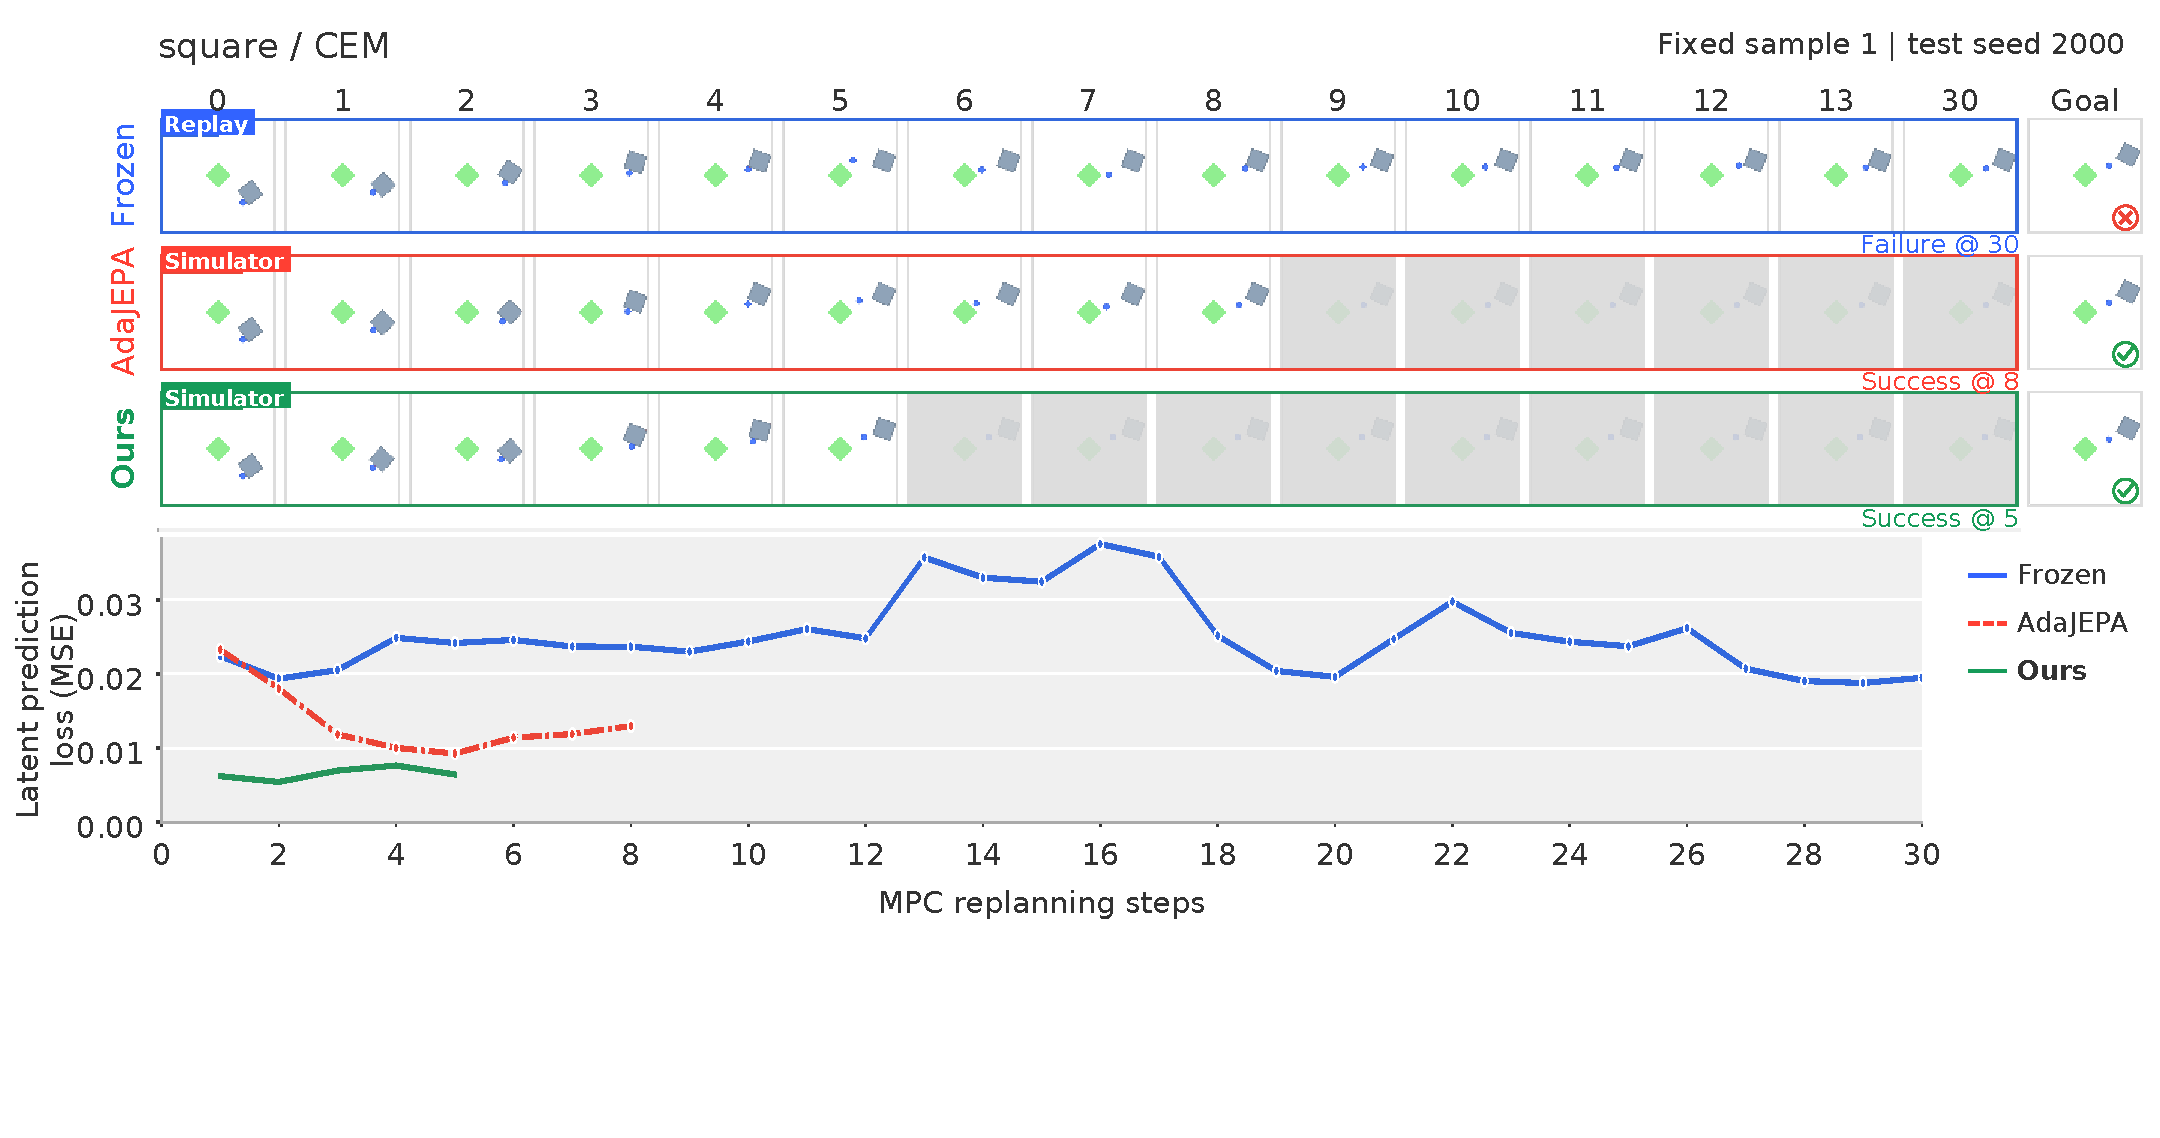
\includegraphics[width=\textwidth]{reference_square.pdf}
 \caption{\textbf{Unseen-square planning under CEM.} Frames show replans 0--13 and 30, then the goal. \ours succeeds at replan 5 and AdaJEPA at 8; Frozen exhausts 30. Gray frames hold terminal states. In both examples, curves end at termination and show each method's visual/proprioceptive prediction MSE over up to five recent transitions.}
 \label{fig:full_shape}
\end{figure*}

\begin{figure*}[!t]
 \centering
 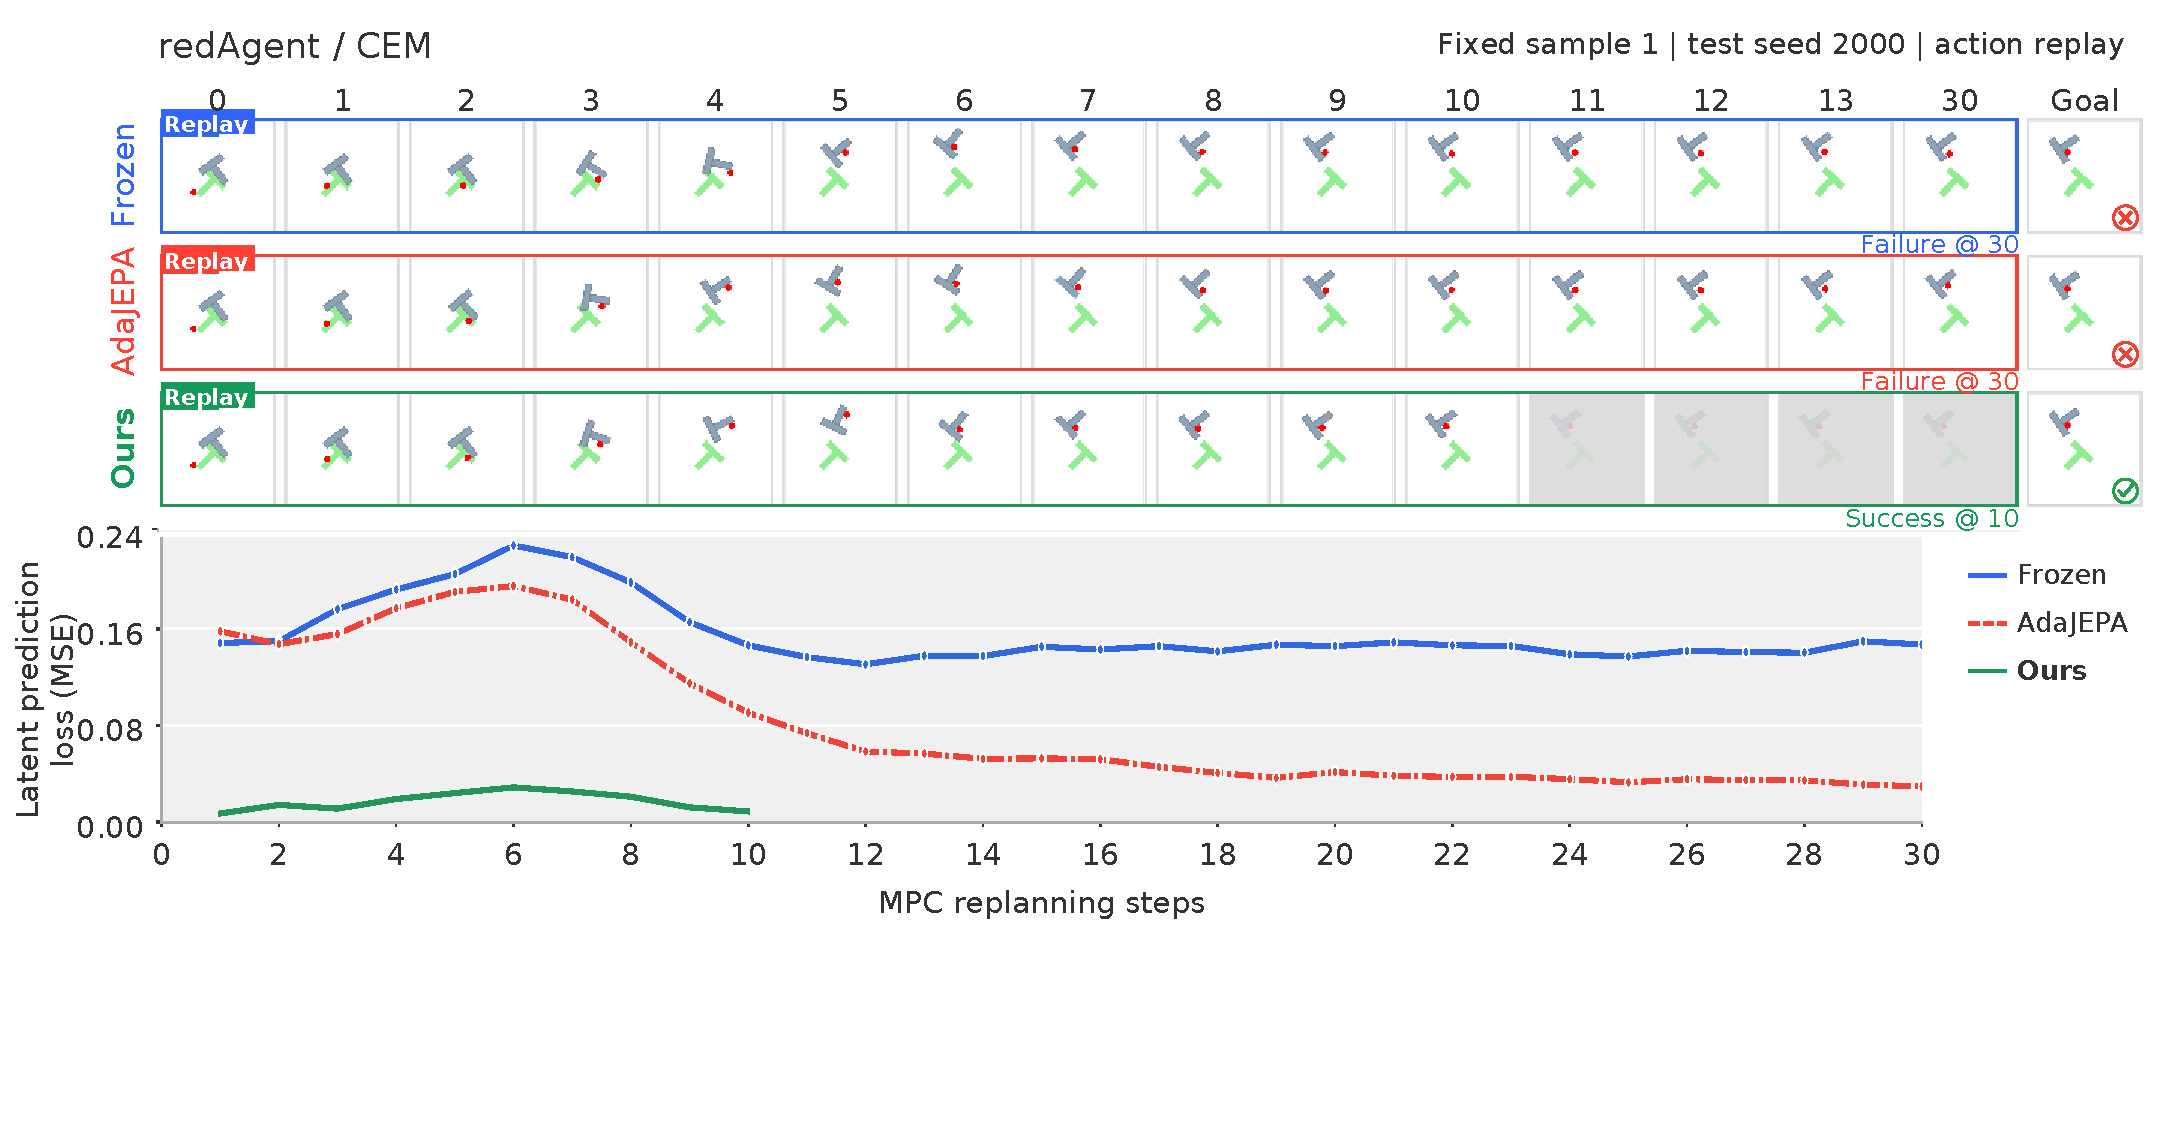
\includegraphics[width=\textwidth]{reference_redagent.pdf}
 \caption{\textbf{Planning through a red-agent appearance shift under CEM.} \ours reaches the goal at replan 10; Frozen and AdaJEPA exhaust 30. Frames replay recorded actions. AdaJEPA's falling prediction loss still leaves the goal unmet.}
 \label{fig:full_visual}
\end{figure*}



The plotted loss is prediction MSE over up to five recent transitions in the visual and proprioceptive latents, excluding action dimensions. Each curve is evaluated with its own method's weights, so absolute loss levels are not directly comparable across methods. The curves show how each method's prediction error changes during execution; task success is the common measure of planning performance. In particular, AdaJEPA reduces its prediction loss on the red-agent episode but still misses the target, whereas \ours achieves the desired configuration.

\subsection{Deformable rollout sequences}
\paperxref{Figure}{fig:deform_reference}{} shows two complete deformable sequences: rope example 1 and granular example 2. Each row contains the start, every third push, and the goal within the same 15-push budget. These instances come from the repeated 50-instance stream and were selected to illustrate episodes with lower final CD for the consolidated predictor than for both baselines. The examples use the third-pass slow predictor without within-episode adaptation; \paperxref{Table}{main-tab:main}{} reports fourth-pass aggregates. DINO-WM frames replay recorded actions in FleX; AdaJEPA and \ours frames were saved during planning. Final CDs come from run logs.

The first rope example starts at CD 1.72. Both baselines finish at 1.54, while \ours reaches 0.31. In granular example 2, final CD is 0.33 for both baselines and 0.14 for \ours. The sequences show how replayed experience improves the geometry of the final configuration under a common action budget, even with fast adaptation disabled.

\begin{figure*}[p]
 \centering
 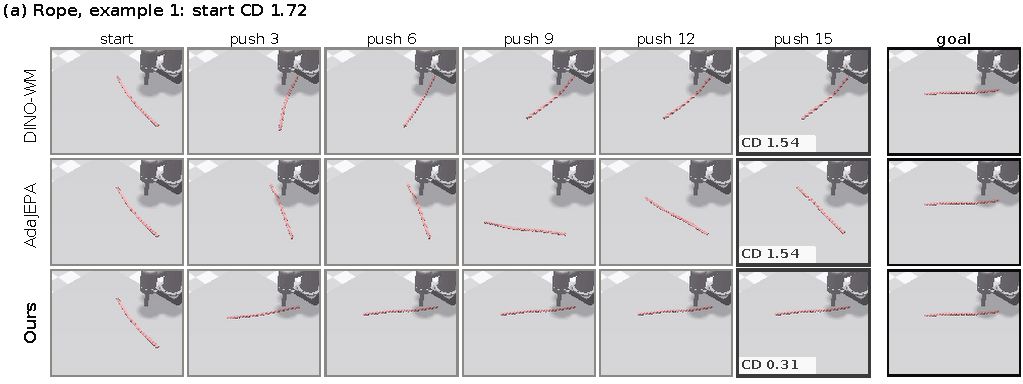
\includegraphics[width=\textwidth]{reference_rope.pdf}
 \par\medskip
 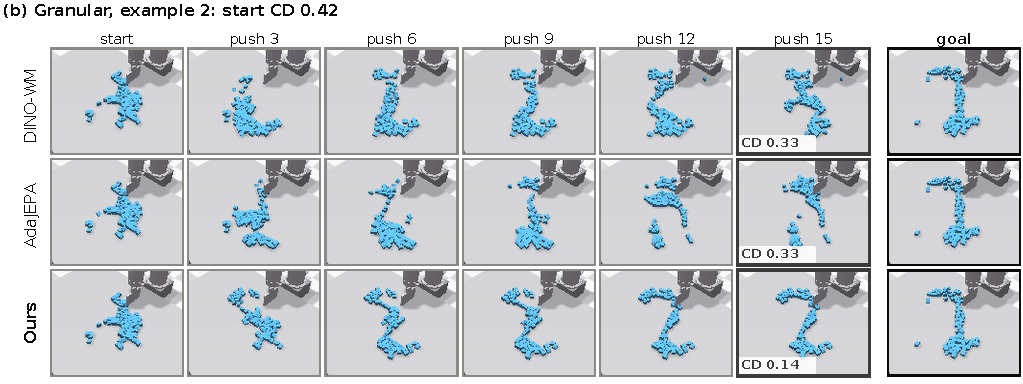
\includegraphics[width=\textwidth]{reference_granular.pdf}
 \caption{\textbf{Rope and granular execution sequences.} Top: rope example 1. Bottom: granular example 2. All methods share the initial configuration and goal. Columns show pushes 0, 3, 6, 9, 12 and 15, then the goal. Final-frame labels report CD (lower is better).}
 \label{fig:deform_reference}
\end{figure*}

\clearpage
{\small
% Keep bibliography endings substantial without altering entry wording.
    \let\standardthebibliography\thebibliography
    \renewcommand{\thebibliography}[1]{%
      \standardthebibliography{#1}%
      \tolerance=1000\relax
      \setlength{\parfillskip}{0pt plus 0.25\linewidth}%
    }
    \bibliographystyle{ieeenat_fullname}
\bibliography{references}
}
\end{document}
